\documentclass[Royal,times,sageh]{sagej}

\usepackage{moreverb,url,natbib, multirow, tabularx}
\usepackage[colorlinks,bookmarksopen,bookmarksnumbered,citecolor=red,urlcolor=red]{hyperref}



% tightlist command for lists without linebreak
\providecommand{\tightlist}{%
  \setlength{\itemsep}{0pt}\setlength{\parskip}{0pt}}



\usepackage{booktabs}
\usepackage{longtable}
\usepackage{array}
\usepackage{multirow}
\usepackage{wrapfig}
\usepackage{float}
\usepackage{colortbl}
\usepackage{pdflscape}
\usepackage{tabu}
\usepackage{threeparttable}
\usepackage{threeparttablex}
\usepackage[normalem]{ulem}
\usepackage{makecell}
\usepackage{xcolor}


\begin{document}


\setcitestyle{aysep={,}}

\title{ActiveCA: an open data product to obtain impedance functions for
active transportation modes in Canada}

\runninghead{}

\author{Anon1\affilnum{}, Anon2\affilnum{}, Anon3\affilnum{}}

\affiliation{\affilnum{}{}}



\begin{abstract}
This article describes and visualizes the data contained in the
\{ActiveCA\} R data package. \{ActiveCA\} contains open data products
designed to obtain impedance functions for active transportation modes
in Canada, retrieved from the General Social Survey collections from
1986 to 2015. The package provides data tables on walking and cycling
episodes, detailing the trip origins, destinations, and duration of each
episode. The origin and destination categories covers a wide variety of
locations, such as home, work or school, libraries, museums,
restaurants, bars, sports centers, health clinics, place of worship, and
others. Addittionally, the package includes details on the respondent's
region characteristics, specifying wheter they live in a metropolitan
area and their province of residency. \{ActiveCA\} enables users to
calculate the average travel time for each origin-destination
combination for each survey year, considering the two active
transportation modes: walking and cycling. For each Census Metropolitan
and Agglomeration Area, we estimated distance decay curves (impedance
functions) for each origin-destination. The package will continue to
expand with contributions from the authors and the broader community
through requests in the future. \{ActiveCA\} is freely accessible for
exploration and download from the associated Github repository, where
the documentation and code involved in creating and manipulating data
and all open data products are detailed.
\end{abstract}

\keywords{Active; mobility; walking; cycling; travel time; impedance;
transportation; R}

\maketitle

\hypertarget{introduction}{%
\section{Introduction}\label{introduction}}

This manuscript presents the open data product \{ActiveCA\}. Open data
products (ODPs) are the outcome of a transparent process that transforms
raw data (open or not) into analysis-ready data, in which all stages of
development follow open principles. ODPs differ from general open data
due to their high utility, added value and open availability. The
product presented in this document is an \texttt{R} data package that
currently consists of processed data tables retrieved from the General
Social Survey (GSS) collections from 1986 to 2015, to obtain impedance
functions for active transportation modes in Canada.

To create this \texttt{R} data package, we collected the GSS surveys,
cleaned them and processed them to make it ready for analysis. An
\texttt{R} data package contains code, data and documentation in a
standardized collection format that can be installed by \texttt{R} users
via a centralized software repository, such as CRAN (Comprehensive R
Archive Network) and GitHub. Although the GSS surveys are publicly
sourced and managed by Statistic Canada, preparing them for analysis can
be time-consuming, tedious and perhaps not even possible for those who
try, due to a lack of documentation or prior knowledge.

The aim of this paper is to walk readers through the data sets and
invite others to experiment in its uses and applications. \{ActiveCA\}
is freely available on GitHub for all to install and freely use in the
spirit of open and reproducible research. Although \{ActiveCA\} was
designed to obtain impedance functions, we admit and hope that its use
can be adopted in various applications that even go beyond the range of
possibilities we have imagined. Not only the data, but also all the code
documenting the processing methodology is available for consultation and
evaluation in its repository. This package contributes to reducing the
barrier to using the information contained in GSS surveys to provide
data-driven decisions in transportation analysis.

\hypertarget{general-social-survey-gss-collection}{%
\section{General Social Survey (GSS)
collection}\label{general-social-survey-gss-collection}}

In Canada, Statistics Canada produces the General Social Surveys (GSS)
to collect data on social trends in order to track changes in the living
conditions of Canadians and well-being over time. This survey tracks
changes in time and it is used to understand how Canadians spend and
manage their time and what factors contribute to their happiness and
stress. The survey was created in 1985 as a series of independent,
annual, cross-sectional surveys, each covering one topic in depth.
Caregiving, families, time use, social identity, volunteering, and
victimization are among the current themes of the GSS.

The six survey themes listed above are repeated every five years. In
addition to the central topic, each cycle includes new content that
addresses emerging and policy-relevant issues, collecting detailed
socio-demographic information, such as age, gender, education, religion,
ethnicity, income, etc. Time-use surveys collect data on all human
activities and can inform a wide range of policies. In particular, three
key themes have been identified as essential for policymaking and for
which no other data source is adequate: unpaid work and non-market
production, well-being, and gender equality. Leisure time, work-life
balance, health, commuting, culture, and sports are among the other
topics covered by time-use surveys. In addition, statistics Canada has
been conducting time-use surveys at five to seven year intervals since
1986, with the most recent being in 2015 (1986, 1992, 1998, 2005, 2010,
and 2015). The time use collects information on participation of
respondents and time spent on a wide range of day-to-day activities
using a 24-hour retrospective diary. Also, information is collected on
the location of these activities (e.g., at home, at work, etc.) and, for
non-personal activities, the people who were present with the respondent
at the time of the activity.

\hypertarget{the-main-file}{%
\subsection{The Main File}\label{the-main-file}}

The Main File compiles an large array of aggregated data, summarizing
the answers to the questionnaire and derived variables that summarize
the respondents' time use across different activities, locations, and
social interactions. This file documents the time and duration that
respondents allocate to each activity and location. The Main File
provides a overview of daily routines and social dynamics, not focusing
on individual activity episodes. Additionally, this file categorizes
activities into bigger groups and subcategories, enhancing the data's
analytical utility with additional metrics such as total transit time,
duration spent with household members, and counts of activities and
episodes. This file is aggregated and prohibits the direct association
between specific activities with particular locations or companions.

\hypertarget{the-episode-file}{%
\subsection{The Episode File}\label{the-episode-file}}

The Episode File records detailed data for each activity episode
reported by respondents. Each episode entry includes the start and end
times, duration, location, and accompanying social context, informing
when and where activities occurred and with whom. The file distinguishes
itself by focusing on individual episodes rather than respondents, with
the data structured around the numerous activity instances that compose
a respondent's day. Although respondent-specific characteristics are not
included within the Episode File, it is possible to link the Main File
and the Episode File by using an identifiable variable present in both
data sets.

\hypertarget{average-travel-times}{%
\section{Average travel times}\label{average-travel-times}}

\begingroup\fontsize{10}{12}\selectfont

\begin{longtable}[t]{>{}llcccccc}
\caption{\label{tab:ch03-make-table-01}\label{tab:ch03-table-01}Descriptive Analysis of Active Transportation Modes: Walking and Cycling Statistics from 1986 to 2015}\\
\toprule
\multicolumn{2}{c}{ } & \multicolumn{6}{c}{Year} \\
\cmidrule(l{3pt}r{3pt}){3-8}
Mode & Statistic & 1986 & 1992 & 1998 & 2005 & 2010 & 2015\\
\midrule
 & count & 4347 & 1500 & 1670 & 5533 & 4379 & 3251\\
\nopagebreak
 & max & 660 & 300 & 255 & 515 & 480 & 900\\
\nopagebreak
 & mean & 21 & 19 & 11 & 12 & 12 & 17\\
\nopagebreak
 & median & 10 & 10 & 5 & 10 & 8 & 10\\
\nopagebreak
\multirow[t]{-5}{*}{\raggedright\arraybackslash \textbf{Walking}} & min & 1 & 1 & 1 & 0 & 0 & 5\\
\cmidrule{1-8}\pagebreak[0]
 & count & NA & 135 & 119 & 333 & 236 & 245\\
\nopagebreak
 & max & NA & 240 & 90 & 180 & 153 & 120\\
\nopagebreak
 & mean & NA & 31 & 21 & 19 & 21 & 24\\
\nopagebreak
 & median & NA & 20 & 15 & 15 & 15 & 15\\
\nopagebreak
\multirow[t]{-5}{*}{\raggedright\arraybackslash \textbf{Cycling}} & min & NA & 5 & 2 & 1 & 1 & 5\\
\bottomrule
\end{longtable}
\endgroup{}

\begingroup\fontsize{6}{8}\selectfont

\begin{ThreePartTable}
\begin{TableNotes}
\item \textit{Note: } 
\item * The symbols used in this table represent the following: 'Min' denotes the minimum time to reach the destination; 'Max' denotes the maximum time to reach the destination; '(\%)' indicates a percentage of the total time to reach the destination; 'Med' refers to the median time to reach the destination
\end{TableNotes}
\begin{longtable}[t]{ccccc>{}c|ccc>{}c|cccc}
\caption{\label{tab:ch03-make-table-02}\label{tab:ch03-table-02}Comparative Trip Stats by Mode and Destination: 1986, 1992, 1998}\\
\toprule
\multicolumn{2}{c}{ } & \multicolumn{4}{c}{1986} & \multicolumn{4}{c}{1992} & \multicolumn{4}{c}{1998} \\
\cmidrule(l{3pt}r{3pt}){3-6} \cmidrule(l{3pt}r{3pt}){7-10} \cmidrule(l{3pt}r{3pt}){11-14}
\multicolumn{1}{c}{\textbf{Destination}} & \multicolumn{1}{c}{\textbf{Mode*}} & \multicolumn{1}{c}{\textbf{Min*}} & \multicolumn{1}{c}{\textbf{Med*}} & \multicolumn{1}{c}{\textbf{Max*}} & \multicolumn{1}{c}{\textbf{(\%)*}} & \multicolumn{1}{c}{\textbf{Min}} & \multicolumn{1}{c}{\textbf{Med}} & \multicolumn{1}{c}{\textbf{Max}} & \multicolumn{1}{c}{\textbf{(\%)}} & \multicolumn{1}{c}{\textbf{Min}} & \multicolumn{1}{c}{\textbf{Med}} & \multicolumn{1}{c}{\textbf{Max}} & \multicolumn{1}{c}{\textbf{(\%)}}\\
\midrule
Home &  & NA & NA & NA & NA & 5 & 20 & 240 & 55.6 & 2 & 15.0 & 90 & 52.9\\
Work or school & Cycling & NA & NA & NA & NA & 5 & 15 & 45 & 25.9 & 5 & 20.0 & 75 & 29.4\\
Other's home &  & NA & NA & NA & NA & 5 & 10 & 145 & 18.5 & 2 & 10.0 & 80 & 17.6\\
Home &  & 1 & 15 & 330 & 46.4 & 1 & 10 & 300 & 59.5 & 1 & 5.0 & 255 & 51.6\\
Other's home & Walking & 1 & 10 & 660 & 42.3 & 1 & 5 & 135 & 21.3 & 1 & 5.0 & 120 & 28.1\\
\addlinespace
Work or school &  & 1 & 10 & 450 & 11.3 & 2 & 10 & 60 & 19.2 & 1 & 6.5 & 75 & 20.4\\
\bottomrule
\insertTableNotes
\end{longtable}
\end{ThreePartTable}
\endgroup{}

\begingroup\fontsize{6}{8}\selectfont

\begin{ThreePartTable}
\begin{TableNotes}
\item \textit{Note: } 
\item * The symbols used in this table represent the following: 'Min' denotes the minimum time to reach the destination; 'Max' denotes the maximum time to reach the destination; '(\%)' indicates a percentage of the total time to reach the destination; 'Med' refers to the median time to reach the destination
\end{TableNotes}
\begin{longtable}[t]{>{\centering\arraybackslash}p{2cm}>{\centering\arraybackslash}p{0.4cm}>{\centering\arraybackslash}p{0.4cm}>{\centering\arraybackslash}p{0.4cm}>{\centering\arraybackslash}p{0.4cm}>{}c|>{\centering\arraybackslash}p{0.4cm}>{\centering\arraybackslash}p{0.4cm}>{\centering\arraybackslash}p{0.4cm}>{}c|>{\centering\arraybackslash}p{0.4cm}>{\centering\arraybackslash}p{0.4cm}>{\centering\arraybackslash}p{0.4cm}>{\centering\arraybackslash}p{0.4cm}}
\caption{\label{tab:ch03-make-table-03}\label{tab:ch03-table-03}Comparative Trip Statistics by Transportation Mode and Destination: 2005, 2010, and 2015}\\
\toprule
\multicolumn{2}{c}{ } & \multicolumn{4}{c}{2005} & \multicolumn{4}{c}{2010} & \multicolumn{4}{c}{2015} \\
\cmidrule(l{3pt}r{3pt}){3-6} \cmidrule(l{3pt}r{3pt}){7-10} \cmidrule(l{3pt}r{3pt}){11-14}
\multicolumn{1}{>{\centering\arraybackslash}p{2cm}}{\textbf{Destination}} & \multicolumn{1}{>{\centering\arraybackslash}p{0.4cm}}{\textbf{Mode*}} & \multicolumn{1}{>{\centering\arraybackslash}p{0.4cm}}{\textbf{Min*}} & \multicolumn{1}{>{\centering\arraybackslash}p{0.4cm}}{\textbf{Med*}} & \multicolumn{1}{>{\centering\arraybackslash}p{0.4cm}}{\textbf{Max*}} & \multicolumn{1}{>{\centering\arraybackslash}p{0.4cm}}{\textbf{(\%)*}} & \multicolumn{1}{>{\centering\arraybackslash}p{0.4cm}}{\textbf{Min}} & \multicolumn{1}{>{\centering\arraybackslash}p{0.4cm}}{\textbf{Med}} & \multicolumn{1}{>{\centering\arraybackslash}p{0.4cm}}{\textbf{Max}} & \multicolumn{1}{>{\centering\arraybackslash}p{0.4cm}}{\textbf{(\%)}} & \multicolumn{1}{>{\centering\arraybackslash}p{0.4cm}}{\textbf{Min}} & \multicolumn{1}{>{\centering\arraybackslash}p{0.4cm}}{\textbf{Med}} & \multicolumn{1}{>{\centering\arraybackslash}p{0.4cm}}{\textbf{Max}} & \multicolumn{1}{>{\centering\arraybackslash}p{0.4cm}}{\textbf{(\%)}}\\
\midrule
Home &  & 1 & 15.0 & 180 & 48.9 & 1 & 15 & 135 & 50.4 & 5 & 20.0 & 120 & 46.9\\
Work or school & Cycling & 1 & 15.0 & 90 & 21.9 & 1 & 15 & 100 & 24.2 & 5 & 15.0 & 120 & 28.6\\
Grocery store &  & 2 & 10.0 & 30 & 10.2 & 5 & 10 & 75 & 8.9 & 5 & 15.0 & 80 & 6.5\\
Other's home &  & 1 & 15.0 & 35 & 9.0 & 5 & 10 & 45 & 9.3 & 5 & 15.0 & 40 & 5.3\\
Restaurant &  & 5 & 20.0 & 35 & 3.0 & 10 & 15 & 153 & 2.1 & 10 & 17.5 & 60 & 4.1\\
\addlinespace
Sport area &  & NA & NA & NA & NA & NA & NA & NA & NA & 10 & 15.0 & 15 & 2.9\\
Health clinic &  & NA & NA & NA & NA & NA & NA & NA & NA & 10 & 15.0 & 90 & 2.0\\
Outdoors &  & 5 & 15.0 & 45 & 6.0 & 3 & 10 & 115 & 3.8 & 15 & 20.0 & 30 & 1.2\\
Neighbourhood &  & NA & NA & NA & NA & NA & NA & NA & NA & 10 & 30.0 & 45 & 1.2\\
Cultural venues &  & 10 & 12.5 & 15 & 0.6 & 10 & 25 & 30 & 1.3 & 15 & 15.0 & 15 & 0.8\\
\addlinespace
Place of worship &  & 20 & 20.0 & 20 & 0.3 & NA & NA & NA & NA & 15 & 15.0 & 15 & 0.4\\
Home &  & 0 & 10.0 & 515 & 44.4 & 0 & 10 & 270 & 43.6 & 5 & 10.0 & 900 & 45.3\\
Work or school & Walking & 0 & 10.0 & 175 & 17.1 & 0 & 10 & 150 & 15.0 & 5 & 10.0 & 190 & 15.1\\
Grocery store &  & 1 & 10.0 & 90 & 12.5 & 1 & 8 & 105 & 13.2 & 5 & 10.0 & 130 & 11.8\\
Restaurant &  & 0 & 5.0 & 85 & 9.3 & 1 & 5 & 153 & 10.0 & 5 & 10.0 & 120 & 8.4\\
\addlinespace
Other's home &  & 1 & 5.0 & 300 & 11.7 & 0 & 5 & 140 & 11.3 & 5 & 10.0 & 120 & 7.3\\
Sport area &  & NA & NA & NA & NA & NA & NA & NA & NA & 5 & 10.0 & 45 & 3.3\\
Outdoors &  & 1 & 5.0 & 295 & 3.6 & 0 & 10 & 480 & 5.2 & 5 & 10.0 & 135 & 2.8\\
Neighbourhood &  & NA & NA & NA & NA & NA & NA & NA & NA & 5 & 10.0 & 60 & 2.1\\
Cultural venues &  & 5 & 12.5 & 40 & 0.6 & 2 & 10 & 40 & 0.7 & 5 & 10.0 & 40 & 1.5\\
\addlinespace
Place of worship &  & 1 & 10.0 & 30 & 0.8 & 1 & 8 & 60 & 0.9 & 5 & 15.0 & 45 & 1.1\\
Health clinic &  & NA & NA & NA & NA & NA & NA & NA & NA & 5 & 10.0 & 130 & 1.0\\
Business &  & NA & NA & NA & NA & NA & NA & NA & NA & 5 & 10.0 & 30 & 0.2\\
\bottomrule
\insertTableNotes
\end{longtable}
\end{ThreePartTable}
\endgroup{}

\begin{figure}

{\centering 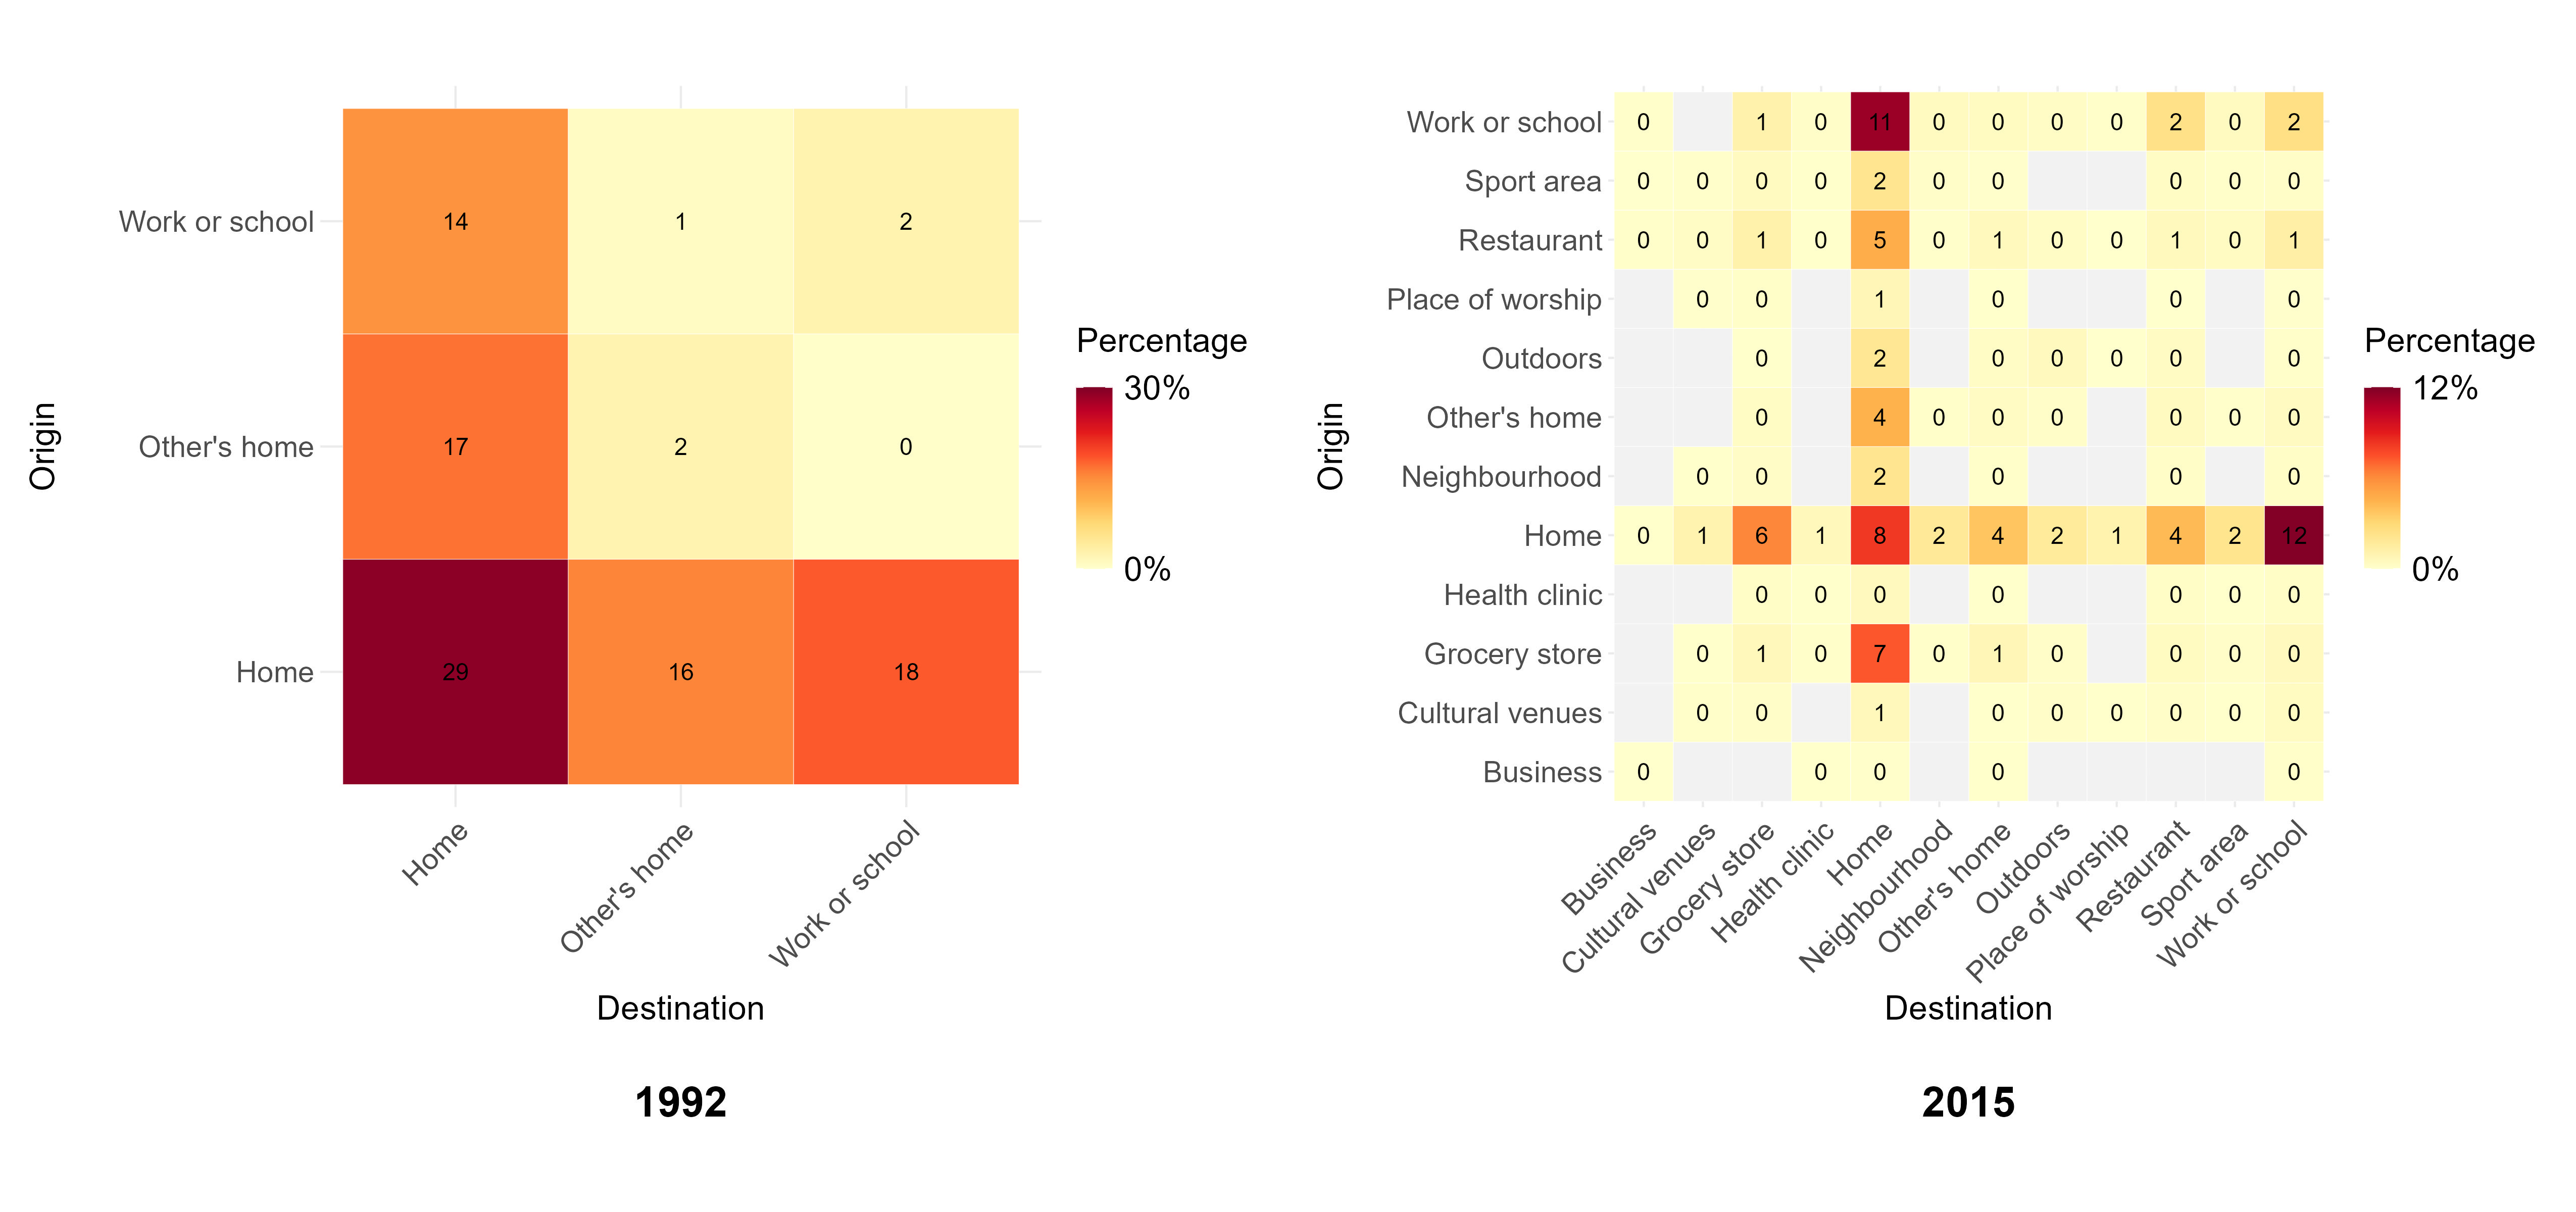
\includegraphics[width=1\linewidth]{Manuscript-figures/walking_hm_fig} 

}

\caption{Percentage of walking Trips Categorized by Origin and Destination}\label{fig:unnamed-chunk-1}
\end{figure}

\begin{figure}

{\centering 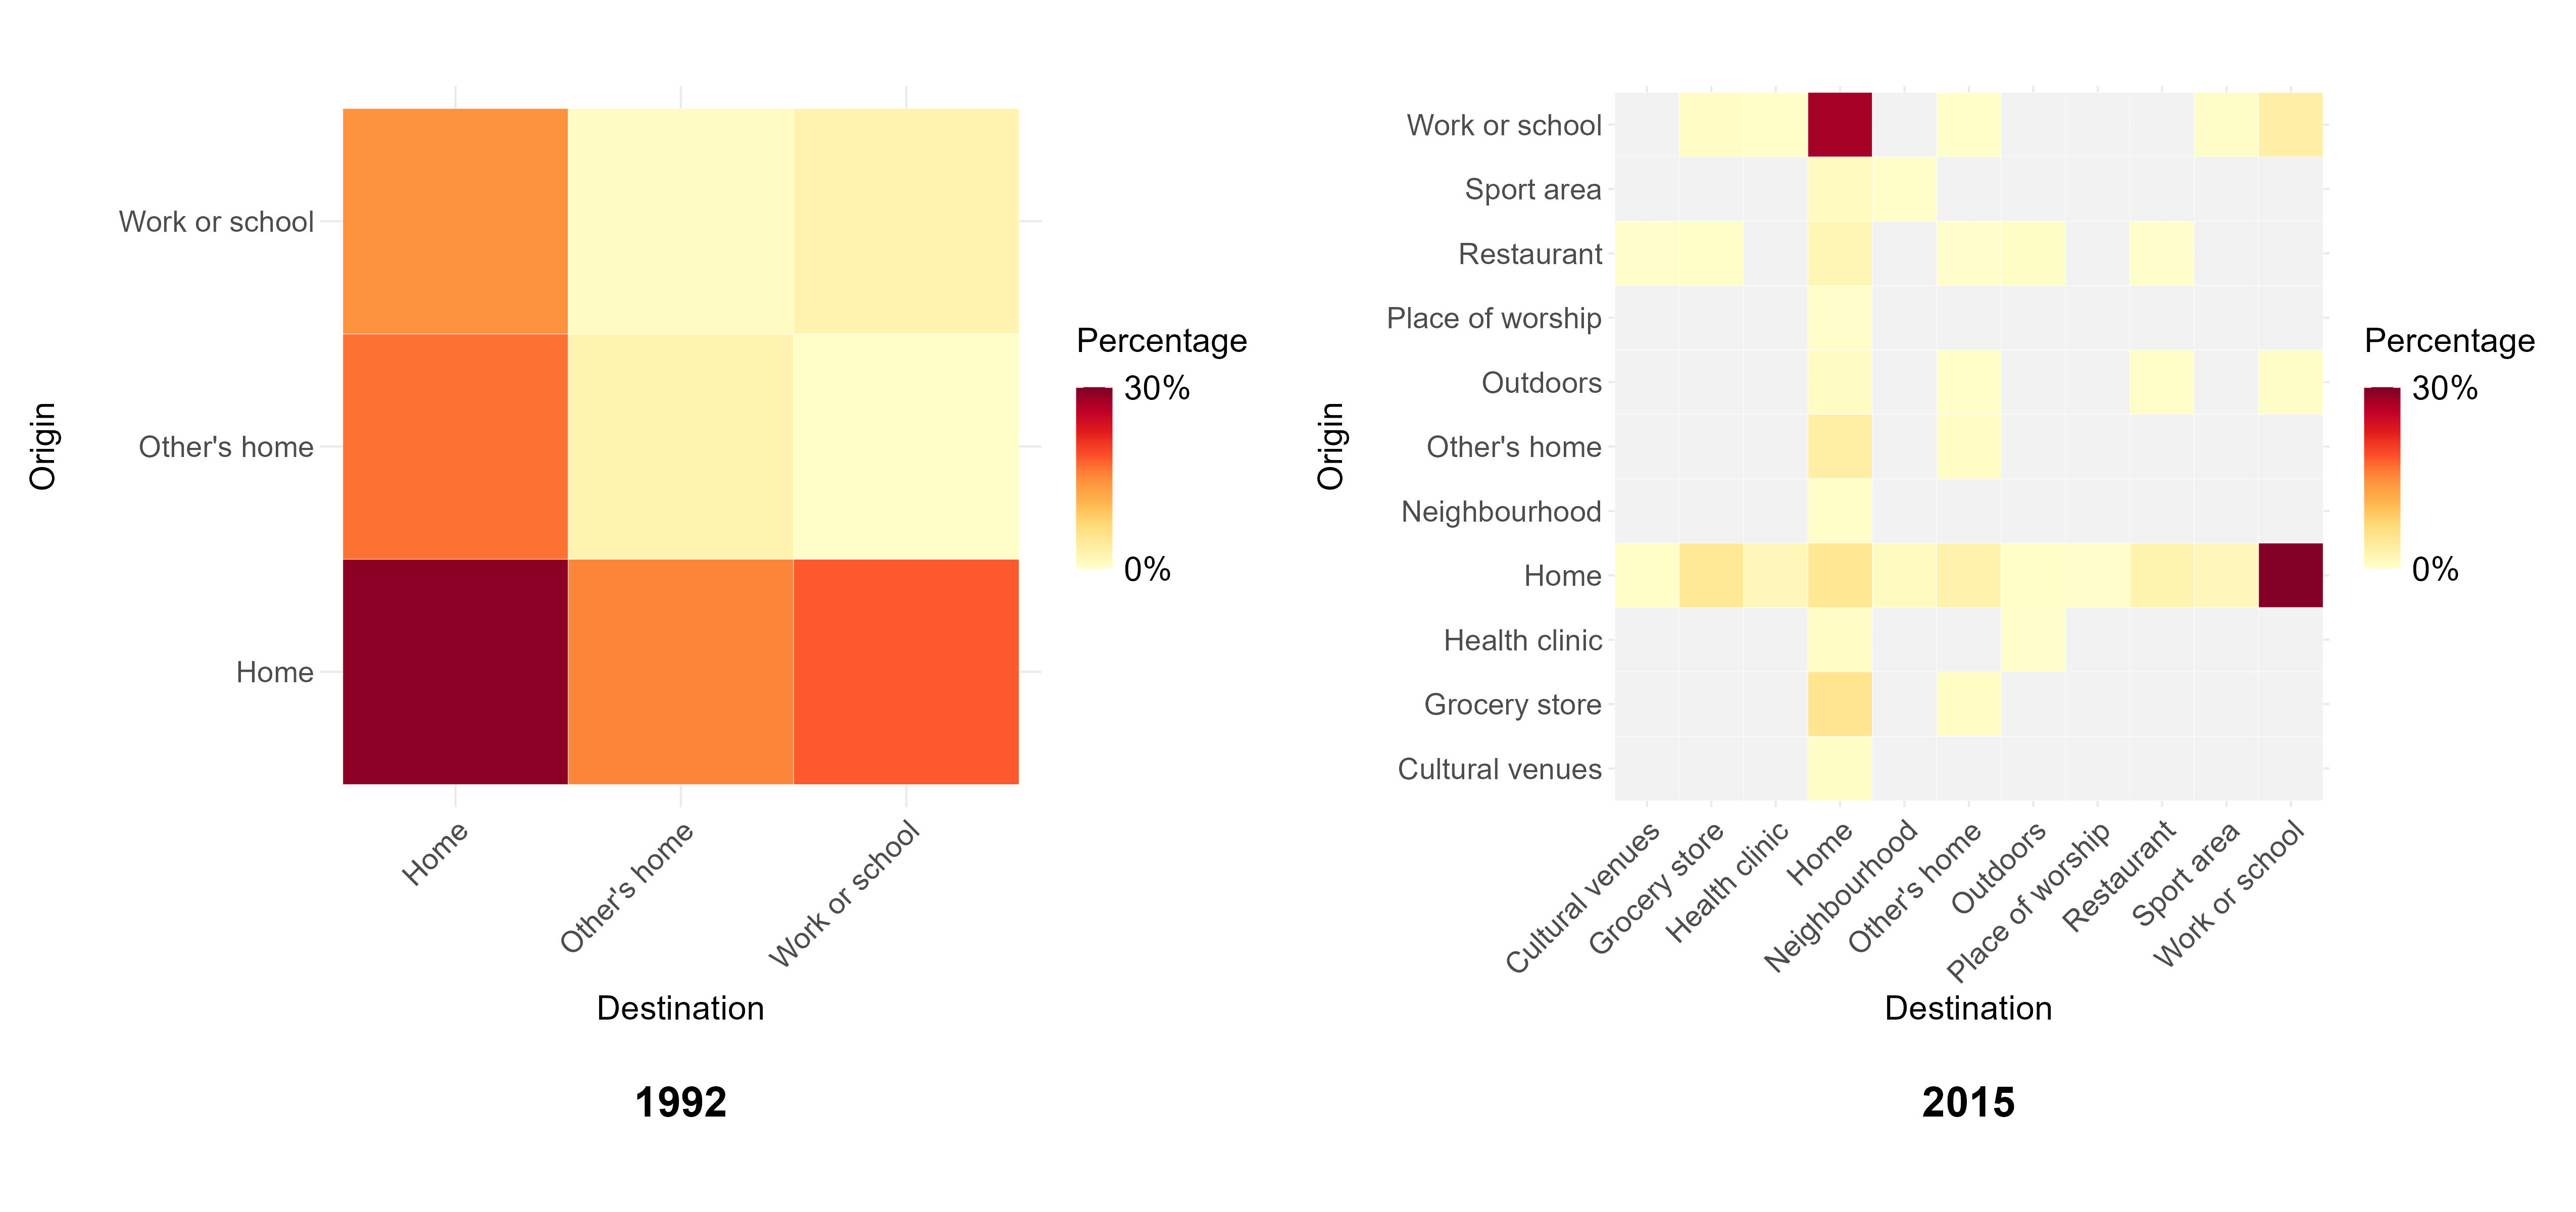
\includegraphics[width=1\linewidth]{Manuscript-figures/cycling_hm_fig} 

}

\caption{Percentage of walking Trips Categorized by Origin and Destination}\label{fig:unnamed-chunk-2}
\end{figure}

\hypertarget{impedance-function-for-canadians-metropolitan-and-census-agglomerations-areas}{%
\section{Impedance function for Canadians Metropolitan and Census
Agglomerations
areas}\label{impedance-function-for-canadians-metropolitan-and-census-agglomerations-areas}}

\begin{table}

\caption{\label{tab:unnamed-chunk-3}\label{tab:ch03-table-04}Impedance functions and selection criteria for walking trips considering 'Work or school' as destination}
\centering
\begin{tabular}[t]{rlrrrrrr}
\toprule
YEAR & f\_name & est\_1 & est\_2 & loglik & aic & bic & count\\
\midrule
2015 & lnorm & 2.55 & 0.64 & -3306028 & 6612061 & 6612069 & 407\\
2010 & lnorm & 2.24 & 0.81 & -2636159 & 5272321 & 5272329 & 367\\
2010 & gamma & 1.99 & 0.18 & -1298182 & 2596367 & 2596373 & 127\\
2005 & lnorm & 2.23 & 0.71 & -1507682 & 3015369 & 3015375 & 224\\
2005 & lnorm & 2.08 & 0.84 & -2565742 & 5131489 & 5131497 & 500\\
\addlinespace
1998 & gamma & 1.23 & 0.09 & -1159374 & 2318752 & 2318758 & 109\\
1992 & lnorm & 2.38 & 0.70 & -1159698 & 2319400 & 2319406 & 113\\
\bottomrule
\end{tabular}
\end{table}

\begin{verbatim}
# A tibble: 7 x 8
   YEAR f_name est_1 est_2   loglik     aic     bic count
  <dbl> <chr>  <dbl> <dbl>    <dbl>   <dbl>   <dbl> <int>
1  2015 lnorm   2.55  0.64 -3306028 6612061 6612069   407
2  2010 lnorm   2.24  0.81 -2636159 5272321 5272329   367
3  2010 gamma   1.99  0.18 -1298182 2596367 2596373   127
4  2005 lnorm   2.23  0.71 -1507682 3015369 3015375   224
5  2005 lnorm   2.08  0.84 -2565742 5131489 5131497   500
6  1998 gamma   1.23  0.09 -1159374 2318752 2318758   109
7  1992 lnorm   2.38  0.7  -1159698 2319400 2319406   113
\end{verbatim}

\hypertarget{concluding-remarks}{%
\section{Concluding remarks}\label{concluding-remarks}}

\bibliographystyle{sageh}
\bibliography{bibfile.bib}


\end{document}
